% AssemblyP1 Beamer talk for microbiology-lab software developers.
% Reproducible build: see talk/README.md and talk/build.sh
\documentclass[10pt,aspectratio=169]{beamer}

\usetheme{default}
\usecolortheme{seahorse}
\setbeamertemplate{navigation symbols}{}
\setbeamertemplate{footline}[frame number]
\setbeamertemplate{itemize item}{\textbullet}

\usepackage[T1]{fontenc}
\usepackage[utf8]{inputenc}
\usepackage{lmodern}
\usepackage{tikz}
\usetikzlibrary{arrows.meta,positioning,fit,backgrounds,shapes}
\usepackage{booktabs}
% NOTE: no \usepackage{xcolor}: beamer already loads it.
% NOTE: beamer already loads hyperref; only tune it.
\hypersetup{hidelinks}

\definecolor{good}{HTML}{1B7A3D}
\definecolor{bad}{HTML}{B02A2A}
\definecolor{accent}{HTML}{1F4E9C}
\definecolor{softbg}{HTML}{EEF2FA}

\newcommand{\takeaway}[1]{%
  \par\smallskip\noindent\textcolor{accent}{\textbf{Takeaway:} #1}}
\newcommand{\verdict}[2]{\textcolor{#1}{\textbf{#2}}}
\newcommand{\code}[1]{\texttt{#1}}

\title{Can ``most likely'' rebuild a genome?}
\subtitle{A 2016 open question, tested to destruction \\ {\small AssemblyP1: bridging vs.\ maximum-likelihood assembly}}
\author{AssemblyP1 Project}
\date{\today}
\institute{\small\url{https://github.com/ottojung/assemblyp1} \quad (Issue \#56 talk)}

\begin{document}

% ================= ACT 1: the problem =================
\begin{frame}[plain]
  \titlepage
  \begin{center}\small For software developers in a microbiology lab. \\
  No biology background, no Lean background assumed.\end{center}
\end{frame}

\begin{frame}{One sentence about DNA}
  \begin{center}
  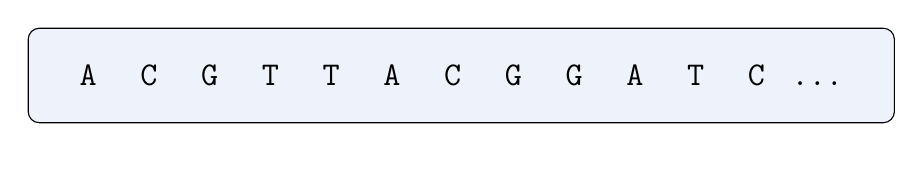
\begin{tikzpicture}[font=\ttfamily\large]
    \node[draw,rounded corners,fill=softbg,minimum width=11cm,minimum height=1.2cm]
      {A \; C \; G \; T \; T \; A \; C \; G \; G \; A \; T \; C \;\dots};
    \node[below=0.15cm of current bounding box, font=\small\normalfont] (lab) {};
  \end{tikzpicture}
  \end{center}
  \vspace{-0.2cm}
  \begin{itemize}
    \item A genome is a \textbf{long string} over \code{A C G T}.
    \item A sequencer returns many \textbf{short strings} (reads).
    \item \textbf{Assembly} = infer the long string from the short ones.
  \end{itemize}
  \takeaway{Think \emph{strings}, not cells. Everything today is strings.}
\end{frame}

\begin{frame}{Assembly, visually: hidden string + scattered reads}
  \begin{center}
  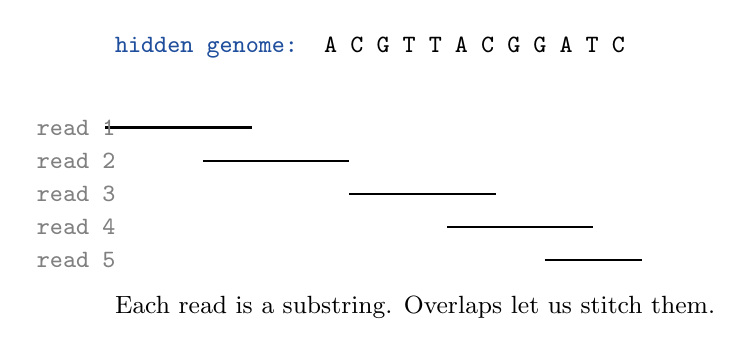
\begin{tikzpicture}[font=\ttfamily\small, x=0.62cm]
    \node[anchor=west] at (0,2.2) {\textcolor{accent}{hidden genome:}~~A C G T T A C G G A T C};
    \foreach \i/\s/\e in {1/0/3,2/2/5,3/5/8,4/7/10,5/9/11} {
      \draw[thick] (\s,1.6-\i*0.42) -- (\e,1.6-\i*0.42);
      \node[anchor=west] at (-1.6,1.6-\i*0.42) {\textcolor{gray}{read \i}};
    }
    \node[anchor=west,font=\small\normalfont] at (0,-1.1)
      {Each read is a substring. Overlaps let us stitch them.};
  \end{tikzpicture}
  \end{center}
  \takeaway{Reads overlap; overlaps are the assembly instructions.}
\end{frame}

\begin{frame}{When nothing repeats, stitching just works}
  \begin{center}
  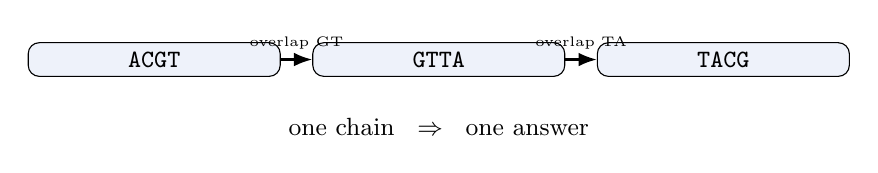
\begin{tikzpicture}[font=\ttfamily\small]
    \node (a) [draw,rounded corners,fill=softbg,minimum width=3.2cm] {ACGT};
    \node (b) [draw,rounded corners,fill=softbg,minimum width=3.2cm,right=0.4cm of a] {GTTA};
    \node (c) [draw,rounded corners,fill=softbg,minimum width=3.2cm,right=0.4cm of b] {TACG};
    \draw[-{Latex},thick] (a) -- (b) node[midway,above,font=\tiny\normalfont] {overlap GT};
    \draw[-{Latex},thick] (b) -- (c) node[midway,above,font=\tiny\normalfont] {overlap TA};
    \node[below=0.4cm of b,font=\small\normalfont] {one chain \;\;$\Rightarrow$\;\; one answer};
  \end{tikzpicture}
  \end{center}
  \takeaway{Unique overlaps give a unique reconstruction. Repeats break this.}
\end{frame}

\begin{frame}{Repeats: the same piece occurs twice}
  \begin{center}
  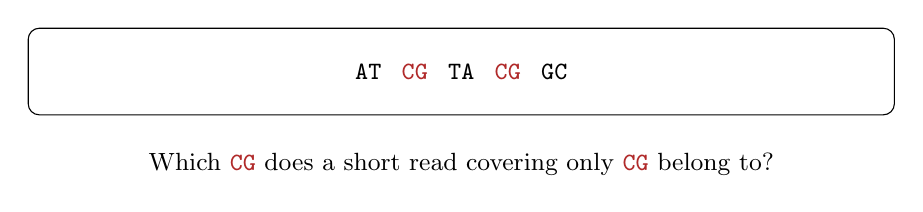
\begin{tikzpicture}[font=\ttfamily\small]
    \node[draw,rounded corners,minimum width=11cm,minimum height=1.1cm] (g)
      {AT \;\textcolor{bad}{\textbf{CG}} \;TA \;\textcolor{bad}{\textbf{CG}} \;GC};
    \node[below=0.1cm of g,font=\small\normalfont\ttfamily\textcolor{bad}{}] {};
    \node[below=0.35cm of g,font=\small\normalfont]
      {Which \textcolor{bad}{\texttt{CG}} does a short read covering only \textcolor{bad}{\texttt{CG}} belong to?};
  \end{tikzpicture}
  \end{center}
  \begin{itemize}
    \item Two placements fit the data equally well.
    \item Real genomes are \textbf{full of repeats} --- this is the core difficulty.
  \end{itemize}
  \takeaway{Repeats create ambiguity: identical substrings, unclear positions.}
\end{frame}

\begin{frame}{A read that \emph{bridges} a repeat settles it}
  \begin{center}
  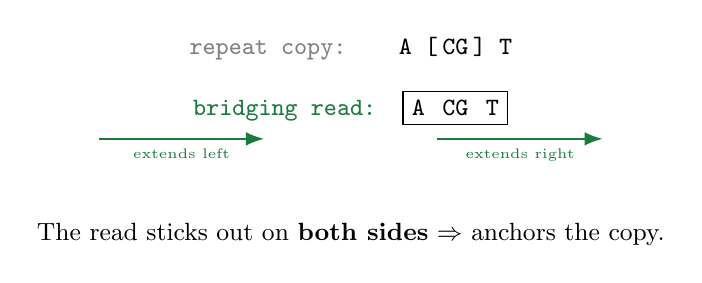
\begin{tikzpicture}[font=\ttfamily\small]
    \node (r1) {\textcolor{gray}{repeat copy:}~~~~A [\,CG\,] T};
    \node[below=0.15cm of r1] (r2) {\textcolor{good}{bridging read:}~~\fbox{A \,\textbf{CG}\, T}};
    \draw[-{Latex},thick,good] (-3.2,-1.15) -- (-1.1,-1.15) node[midway,below,font=\tiny\normalfont] {extends left};
    \draw[-{Latex},thick,good] (1.1,-1.15) -- (3.2,-1.15) node[midway,below,font=\tiny\normalfont] {extends right};
    \node[below=1.0cm of r2,font=\small\normalfont]
      {The read sticks out on \textbf{both sides} $\Rightarrow$ anchors the copy.};
  \end{tikzpicture}
  \end{center}
  \takeaway{Bridging = a read reaches past the repeat on both sides.}
\end{frame}

\begin{frame}{The 2016 deal: bridge everything, recover everything}
  \begin{block}{Shomorony et al.\ (2016), informally}
    If the reads cover the genome, \textbf{every triple repeat} is fully bridged,
    and every \textbf{interleaved repeat pair} is bridged\dots
  \end{block}
  \begin{center}
  \dots then their \textbf{Not-So-Greedy} algorithm recovers the true circular genome (up to rotation).
  \end{center}
  \takeaway{Structural reconstructibility: enough bridging $\Rightarrow$ exact recovery.}
\end{frame}

% ================= ACT 2: the question =================
\begin{frame}{The open question: does ``most likely'' agree?}
  \begin{block}{The 2016 sentence}
    Do bridging conditions also guarantee that the
    \textbf{maximum-likelihood sequence is the true sequence}?
  \end{block}
  \begin{itemize}
    \item Likelihood from Medvedev--Brudno (2009): which candidate genome
      makes the observed reads \textbf{most probable}?
    \item Two algorithms, same input --- do they agree?
  \end{itemize}
  \takeaway{A natural conjecture: reconstructible $\Rightarrow$ most likely.}
\end{frame}

\begin{frame}{Maximum likelihood in one picture}
  \begin{center}
  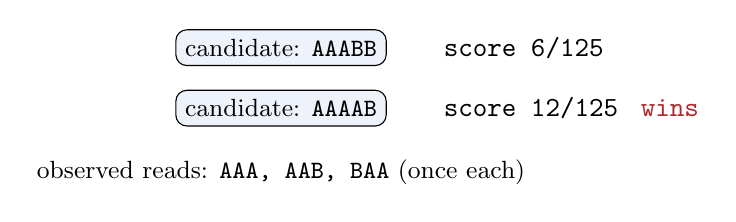
\begin{tikzpicture}[font=\small]
    \node[draw,rounded corners,fill=softbg] (t) {candidate: \texttt{AAABB}};
    \node[draw,rounded corners,fill=softbg,below=0.3cm of t] (d) {candidate: \texttt{AAAAB}};
    \node[right=0.6cm of t,font=\ttfamily] {score 6/125};
    \node[right=0.6cm of d,font=\ttfamily] {score 12/125 \;\textcolor{bad}{wins}};
    \node[below=0.3cm of d,font=\small] {observed reads: \texttt{AAA, AAB, BAA} (once each)};
  \end{tikzpicture}
  \end{center}
  \begin{itemize}
    \item Score = probability the candidate would emit exactly these read counts.
    \item Pick the highest score. Sounds obviously right\dots
  \end{itemize}
  \takeaway{ML = ``which genome would most plausibly have produced these reads?''}
\end{frame}

\begin{frame}{Why the question was interesting}
  \begin{itemize}
    \item Two philosophies: \textbf{combinatorial} (bridge the repeats)
      vs.\ \textbf{statistical} (maximize likelihood).
    \item If they coincide, one condition serves both --- elegant and practical.
    \item Nobody knew. It stayed open for a decade.
  \end{itemize}
  \takeaway{Unifying two worldviews was the prize.}
\end{frame}

\begin{frame}{A trap: the question hides four ambiguities}
  \begin{enumerate}
    \item \textbf{Which likelihood?} exact counts vs.\ binomial approximation vs.\ flow.
    \item \textbf{Which reads?} oriented strings vs.\ reverse-complement molecules.
    \item \textbf{Which candidates?} any length, or only the true length?
    \item \textbf{Which claim?} truth \emph{is} a maximizer vs.\ truth is the \emph{unique} maximizer.
  \end{enumerate}
  \takeaway{One English sentence, a family of theorems. We split them instead of guessing.}
\end{frame}

% ================= ACT 3: finite results =================
\begin{frame}{Spoiler: the finite answer is ``sometimes''}
  \begin{center}
  \begin{tabular}{@{}lll@{}}
    \toprule
    Setting & Verdict \\
    \midrule
    Same length, oriented, flow candidates & \verdict{good}{TRUE --- unique} \\
    Exact counts, any length & \verdict{bad}{FALSE} \\
    Binomial approximation, any length & \verdict{bad}{FALSE} \\
    Molecule (reverse-complement) flow & \verdict{bad}{FALSE} \\
    Population (infinite reads), repaired & \verdict{good}{TRUE --- unique} \\
    \bottomrule
  \end{tabular}
  \end{center}
  \takeaway{The map, up front. Now: \emph{why} each row holds.}
\end{frame}

\begin{frame}{How the truth loses: multiplicity reallocation}
  \begin{center}
  Truth \texttt{AAABB}: spectrum \{\texttt{AAA}:1, \texttt{AAB}:1, \texttt{BAA}:1\} \\
  Rival \texttt{AAAAB}: spectrum \{\texttt{AAA}:\textbf{2}, \texttt{AAB}:1, \texttt{BAA}:1\}
  \end{center}
  \begin{itemize}
    \item Reads observed once each; rival doubles down on the seen type \texttt{AAA}.
    \item Likelihood ratio $= 2 > 1$. The wrong genome wins \textbf{strictly}.
    \item Bridging still holds (checked): repeats are bridged, coverage holds.
  \end{itemize}
  \takeaway{The rival bets harder on what was observed --- and the bet pays off.}
\end{frame}

\begin{frame}{Repeat the lucky read, amplify the failure}
  \begin{center}
  \begin{tabular}{@{}ll@{}}
    \toprule
    Observations & likelihood ratio (rival / truth) \\
    \midrule
    \texttt{AAA, AAB, BAA} & $2$ \\
    \texttt{AAA}$\times$2\texttt{, AAB, BAA} & $4$ \\
    \texttt{AAA}$\times$k\texttt{, AAB, BAA} & $2^{k}$ \\
    \bottomrule
  \end{tabular}
  \end{center}
  \takeaway{Not a tie, not a rounding error --- a one-parameter family of failures.}
\end{frame}

\begin{frame}{The surprise: one slice is completely safe}
  \begin{block}{Rigidity theorem (same length, oriented)}
    Under bridging, the truth's read-type spectrum is the \textbf{only}
    positive circulation on its window graph. No strict rival exists ---
    for \textbf{any} genome length, read length, or alphabet.
  \end{block}
  \begin{itemize}
    \item Only the triple-repeat clause is even needed.
    \item Same observation $\Rightarrow$ same score: ratio exactly 1.
    \item Plus a classical uniqueness input: same spectrum $\Rightarrow$ same genome up to rotation.
  \end{itemize}
  \takeaway{On this slice the truth isn't just \emph{a} winner --- it's the \emph{only} winner.}
\end{frame}

\begin{frame}{Why ``same length'' is suspicious}
  \begin{itemize}
    \item The safe slice assumes candidates have the \textbf{true length}.
    \item Real assemblers don't know the true length in advance.
    \item Drop the assumption: rival \texttt{AAAATT} (length 6) beats truth
      \texttt{AAATT} (length 5) with one extra \texttt{AAA} observation.
  \end{itemize}
  \begin{center}
  \begin{tabular}{@{}lll@{}}
    \toprule
    extra \texttt{AAA}s & exact & binomial \\
    \midrule
    0 & truth wins & truth wins \\
    1 & \verdict{bad}{rival wins} & \verdict{bad}{rival wins} \\
    \bottomrule
  \end{tabular}
  \end{center}
  \takeaway{Knowledge of the true length does real work --- and we don't have it.}
\end{frame}

\begin{frame}{Even intrinsic checks can't fix finite luck}
  \begin{itemize}
    \item Try: restrict candidates by \textbf{their own} repeat structure (P1/P2),
      no privileged true length.
    \item Still fails: truth \texttt{AABBC} vs.\ shorter rival \texttt{AABC},
      both structurally clean, unlucky sample \texttt{\{AAB, BCA\}}.
    \item Ratio $25/16 > 1$. The sample, not the structure, is at fault.
  \end{itemize}
  \takeaway{Two failure modes: \textbf{structural} ambiguity vs.\ \textbf{sampling} fluctuation.}
\end{frame}

% ================= ACT 4: population repair =================
\begin{frame}{The repair: infinite reads remove the luck}
  \begin{itemize}
    \item Replace the finite sample by its \textbf{population limit}:
      the true read distribution.
    \item Score candidates against the distribution, not the draw.
  \end{itemize}
  \begin{block}{Gibbs / KL identity}
    Truth always maximizes population likelihood; a rival ties
    \textbf{iff} its read distribution equals the truth's.
  \end{block}
  \takeaway{Maximizer statement becomes free. Uniqueness = ``same distribution $\Rightarrow$ same genome''.}
\end{frame}

\begin{frame}{Population uniqueness: the repaired theorem}
  \begin{block}{Strongest current positive result (plain English)}
    Among primitive, structurally clean (P2) oriented circular candidates,
    the true genome is the \textbf{unique} population-maximum-likelihood
    genome, up to rotation.
  \end{block}
  \begin{itemize}
    \item Step 1 (free): Gibbs identity $\Rightarrow$ truth is a maximizer.
    \item Step 2 (project): primitivity + P2 turns equal distributions into equal spectra.
    \item Step 3 (classical): Bresler--Bresler--Tse uniqueness turns equal spectra into equal genomes.
  \end{itemize}
  \takeaway{Cleaner question, clean answer --- but it does \emph{not} settle the 2016 finite question.}
\end{frame}

% ================= ACT 5: how it was done =================
\begin{frame}{How the work was actually done}
  \begin{center}
  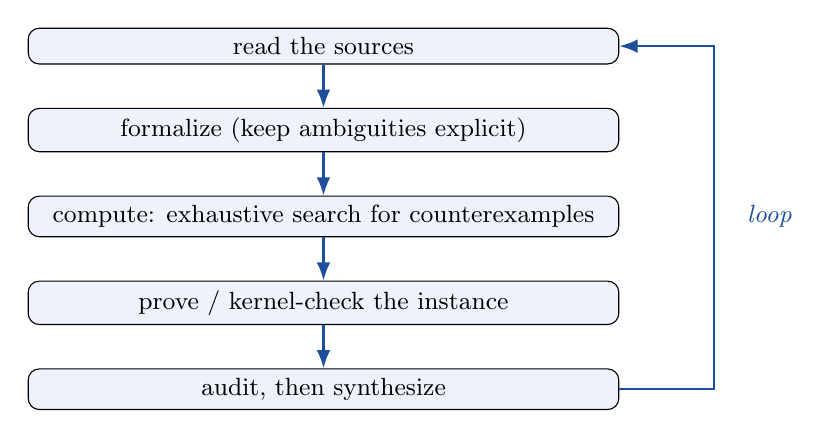
\begin{tikzpicture}[font=\small, node distance=0.55cm,
      box/.style={draw,rounded corners,fill=softbg,minimum width=7.5cm,align=center}]
    \node[box] (a) {read the sources};
    \node[box,below=of a] (b) {formalize (keep ambiguities explicit)};
    \node[box,below=of b] (c) {compute: exhaustive search for counterexamples};
    \node[box,below=of c] (d) {prove / kernel-check the instance};
    \node[box,below=of d] (e) {audit, then synthesize};
    \draw[-{Latex},thick,accent] (a) -- (b);
    \draw[-{Latex},thick,accent] (b) -- (c);
    \draw[-{Latex},thick,accent] (c) -- (d);
    \draw[-{Latex},thick,accent] (d) -- (e);
    \draw[-{Latex},thick,accent] (e.east) -- ++(1.2,0) |- (a.east);
    \node[right=1.5cm of c,font=\small\itshape,text=accent] {loop};
  \end{tikzpicture}
  \end{center}
  \takeaway{Source reading $\to$ formalization $\to$ computation $\to$ proof $\to$ audit $\to$ synthesis.}
\end{frame}

\begin{frame}{Four levels of ``we checked it''}
  \begin{center}
  \begin{tabular}{@{}ll@{}}
    \toprule
    Level & what it buys you \\
    \midrule
    Empirical test & works on these inputs \\
    Exact computation & exact arithmetic on this instance \\
    Mathematical proof & works for all inputs (human-checked) \\
    Lean kernel check & proof re-verified by a tiny trusted checker \\
    \bottomrule
  \end{tabular}
  \end{center}
  \begin{itemize}
    \item Pipeline: \textbf{Python finds} a candidate $\to$ \textbf{Lean proves}
      this exact instance breaks (or holds) the claim.
  \end{itemize}
  \takeaway{Search discovers; Lean certifies. Different jobs, both needed.}
\end{frame}

\begin{frame}{What Lean actually does (30 seconds)}
  \begin{itemize}
    \item Lean is a \textbf{proof assistant}: you state a proposition,
      write a proof, and a small trusted \textbf{kernel} re-checks every step.
    \item Stronger than ``the script ran'': the certificate is mathematics,
      not test coverage.
    \item Example: \code{FixedLengthExactCounterexample} proves
      ``this \texttt{AAABB}/\texttt{AAAAB} instance satisfies bridging
      \emph{and} the likelihood inequality is strictly $> 1$''.
  \end{itemize}
  \takeaway{Computation says ``look here''; the kernel says ``this instance truly counts''.}
\end{frame}

\begin{frame}{Process lessons worth stealing}
  \begin{itemize}
    \item \textbf{Split, don't guess:} four ambiguous axes became explicit variants.
    \item \textbf{Strict beats tied:} strict $>$ inequalities survive every tie convention.
    \item \textbf{Negatives transfer up:} a same-length counterexample kills the general claim.
    \item \textbf{Keep failures:} a gapped proof attempt is documented, with the killing example.
    \item \textbf{Issues as roadmap:} each research question is a trackable unit.
  \end{itemize}
  \takeaway{Epistemic hygiene --- source fact vs.\ project choice vs.\ proved vs.\ computed --- prevented false victories.}
\end{frame}

\begin{frame}{What remains open}
  \begin{itemize}
    \item The published sentence's intended reading is still partly ambiguous
      (objective, strand convention, length, maximizer vs.\ uniqueness).
    \item One finite slice stays open: per-occurrence Section~6.2 strengthening.
    \item Population result is oriented-only; molecule version unaddressed.
    \item The finite 2016 question $\neq$ the repaired population result.
  \end{itemize}
  \takeaway{Honest boundary: proved, refuted, and still-open are labeled --- see the white paper ledger.}
\end{frame}

\begin{frame}{Closing: the story in one minute}
  \begin{enumerate}
    \item Assembly = rebuild a hidden string from overlapping reads; \textbf{repeats} cause ambiguity.
    \item \textbf{Bridging} reads anchor repeats; in 2016 that sufficed for reconstruction.
    \item The question: does it also imply \textbf{maximum-likelihood} recovery? Tempting.
    \item Finite answer: \textbf{no, in general} --- small strict counterexamples (kernel-checked).
    \item One safe slice: \textbf{same-length oriented} --- unique recovery up to rotation.
    \item True length was load-bearing; intrinsic checks still lose to \textbf{sampling luck}.
    \item \textbf{Population} likelihood removes luck: unique recovery under primitivity + P2.
    \item Method: split ambiguities, search computationally, certify in Lean, audit failures.
  \end{enumerate}
\end{frame}

\begin{frame}[plain]
  \begin{center}
    {\Large Thank you.} \\[0.4em]
    White paper + proofs + certificates:
    \url{https://github.com/ottojung/assemblyp1} \\[0.4em]
    {\small Shomorony et al.\ 2016 \;\;$\cdot$\;\; Medvedev--Brudno 2009
    \;\;$\cdot$\;\; Bresler--Bresler--Tse 2013}
  \end{center}
\end{frame}

\appendix

\begin{frame}{Backup: the likelihood formulas}
  \small
  Exact multinomial (uses candidate's own length $|D|$):
  \[ \mathcal{L}_{\mathrm{ex}}(D;x) = \frac{n!}{\prod_w x(w)!}
     \prod_{w} \left(\frac{\mathrm{spec}_L(D)(w)}{|D|}\right)^{x(w)} \]
  Fixed-length binomial (external size $N$):
  \[ \mathcal{L}_{\mathrm{bin}}(D;x) = \prod_w \binom{n}{x(w)}
     \left(\frac{\mathrm{spec}_L(D)(w)}{N}\right)^{x(w)}
     \left(1-\frac{\mathrm{spec}_L(D)(w)}{N}\right)^{n-x(w)} \]
  Population (infinite reads): $\ell_S(D) = \sum_w p_S(w)\log p_D(w)$.
\end{frame}

\begin{frame}{Backup: why circular genomes?}
  \begin{itemize}
    \item The 2016 exposition uses \textbf{circular} strings to avoid edge effects:
      every position has the same read distribution.
    \item Rotation symmetry is then unavoidable: a rotated genome has an
      identical spectrum, so ``up to cyclic shift'' is the finest possible claim.
    \item Error-free, fixed-length reads are the same kind of idealization:
      they isolate repeat ambiguity from noise.
  \end{itemize}
\end{frame}

\begin{frame}{Backup: oriented vs.\ molecule reads}
  \begin{itemize}
    \item \textbf{Oriented:} a read is the string as seen on one strand.
    \item \textbf{Molecule:} a read and its reverse complement are the same observation.
    \item Collapsing strands \emph{creates} multiplicity the data doesn't force ---
      a separate failure mechanism with its own counterexamples.
  \end{itemize}
\end{frame}

\begin{frame}{Backup: references}
  \footnotesize
  \begin{itemize}
    \item Shomorony, Kim, Courtade, Tse. ``Information-optimal genome assembly
      via sparse read-overlap graphs.'' \textit{Bioinformatics} 32(17), 2016.
    \item Medvedev, Brudno. ``Maximum likelihood genome assembly.''
      \textit{J.\ Comput.\ Biol.} 16(8), 2009.
    \item Bresler, Bresler, Tse. ``Optimal assembly for high throughput shotgun
      sequencing.'' BMC Bioinformatics 14(S5), 2013.
    \item Cover, Thomas. \textit{Elements of Information Theory} (Gibbs/KL identity).
    \item AssemblyP1 white paper and epistemic ledger, in-repo (\code{paper/}).
  \end{itemize}
\end{frame}

\end{document}
